\section{Software modules}

The NEW detector will be fully controlled via Labview software with custom modules designed specifically by NEXT. The system consist of 6 software modules which communicate via TCP/IP protocol. The organisation of the modules is as follows:

\begin{itemize}
\item A main module that communicates with all the others and handles all the relevant information.
\item A module to control the voltages in the EL grids.
\item A module to control the power supply of the PMTs.
\item A module to control the SiPMs and front-end electronics.
\item A module to control the gas system.
\item A hybrid module controlling various sensors and the vacuum pump of the energy plane.
\end{itemize}


The modules are currently being tested in the NEW setup.

\subsection{PMTs power supply Slow Control}

This module is in charge of monitoring and controlling the PMT power supply. 
%The module has two ways to set the output voltage for each channel, one with predefined values and the other with an equation for the required PMT gain.

%The module is password protected, nothing can be changed if the password is not set. The message "Wrong password" is shown if the password is incorrect.
%
The actions that it can perform are:
\begin{itemize}
\item When the measured current in one of the PMTs is greater than the maximum set current, a flag on the Labview screen that correspond to that PMT will go off and the power supply channel also will be turned off. After a defined recovery time, the PMT will be turned on again, but if the over-current occurs again the PMT is turned off permanently. 
In any case, if an over-current is measured in a PMT, the module will send a message with the PMT number and the time of the event to the Main Slow Control module to be logged in the general report.
\item If the vacuum level in the vacuum region of the energy plane is less than a threshold, the PMTs will go off and an e-mail will be sent to the team in control. 
\end{itemize}

In addition to e-mail in case of abnormal situations, the module has predefined several predefined diagnostic messages, (e.g, when the module is turned on or off).

Every day, two report files are created with all measurements of the day: one with voltages and the other with the currents. This is logged typically every 30 seconds (the time can be changed by the operator). The contents of the report is voltage or current for each PMT and a timestamp. In the figure  \ref{fig:PMT:REPORT} an example of both reports is given.


\begin{figure}[ht!]
  \centering
  \subfloat[\textit{Voltage}]{\label{fig:PMT:REPORT_V}
  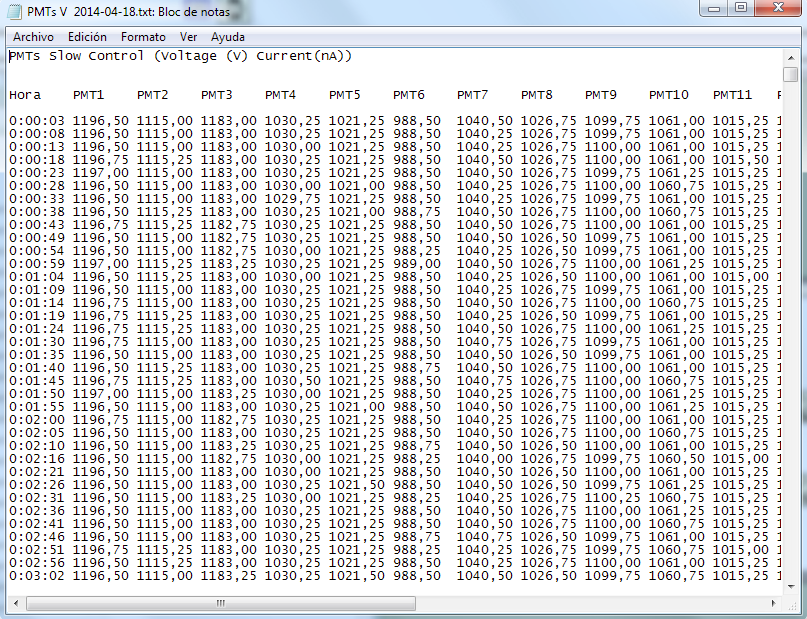
\includegraphics[width=0.5\textwidth]{REPORT_V.png}}   
  %\hspace{5mm}             
  \subfloat[\textit{Current}]{\label{fig:PMT:REPORT_I}
  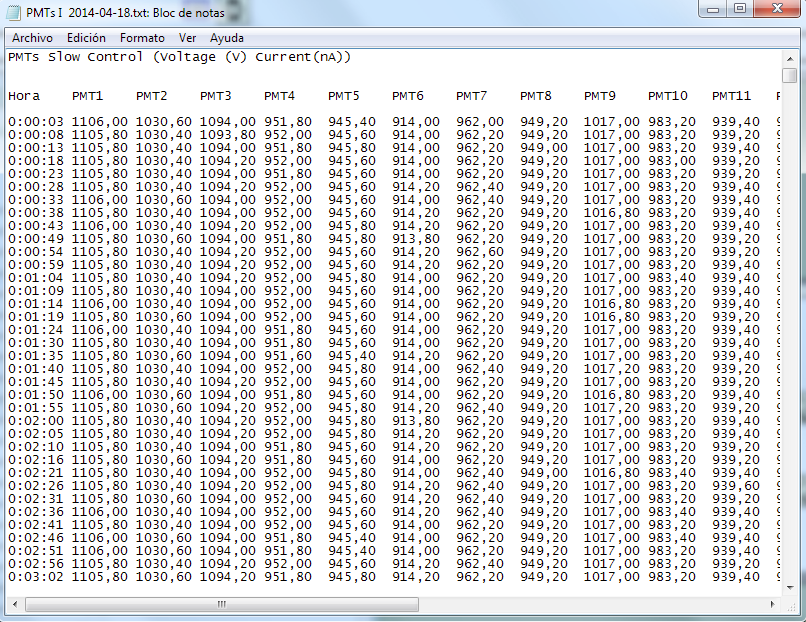
\includegraphics[width=0.5\textwidth]{REPORT_I.png}}
  \caption{\textit{Examples of voltage and current reports}}
  \label{fig:PMT:REPORT}
\end{figure}


The module will send messages for the following events:

\begin{itemize}
\item Turning on or turning off the PMTs.
\item Over-current in a PMT.
\item Other software module asks for a status update.
\end{itemize}

\vspace{2cm}

The visible part of the module is distributed over four pages:

\begin{itemize}
\item Main page.
\item Control.
\item Module data.
\item TCP/IP
\end{itemize}

The contents of each page in the PMT slow control module are described below:

\subsubsection*{Main page}

The main page shows the voltage that is set in each PMT and the voltage and current measured continuously plotted on a chart voltage or current versus time. Also if a trip occurs in a PMT the flag that corresponds to that PMT is illuminated in red indicating that the PMT is tripping.

This module communicates with the Grids High Voltage, Sensors and Main Slow Control modules. If the link is up and there are no failures the indicators are green, otherwise the indicator are in grey.

The voltage of each PMT can be set with predefined values or with an equation for a specific gain.

Figure \ref{fig:PMT:MAIN} shows a screenshot with the main page of the module.

\begin{figure}[ht!]
    \bigskip
    \begin{center}\leavevmode
        \rotatebox{0}{
        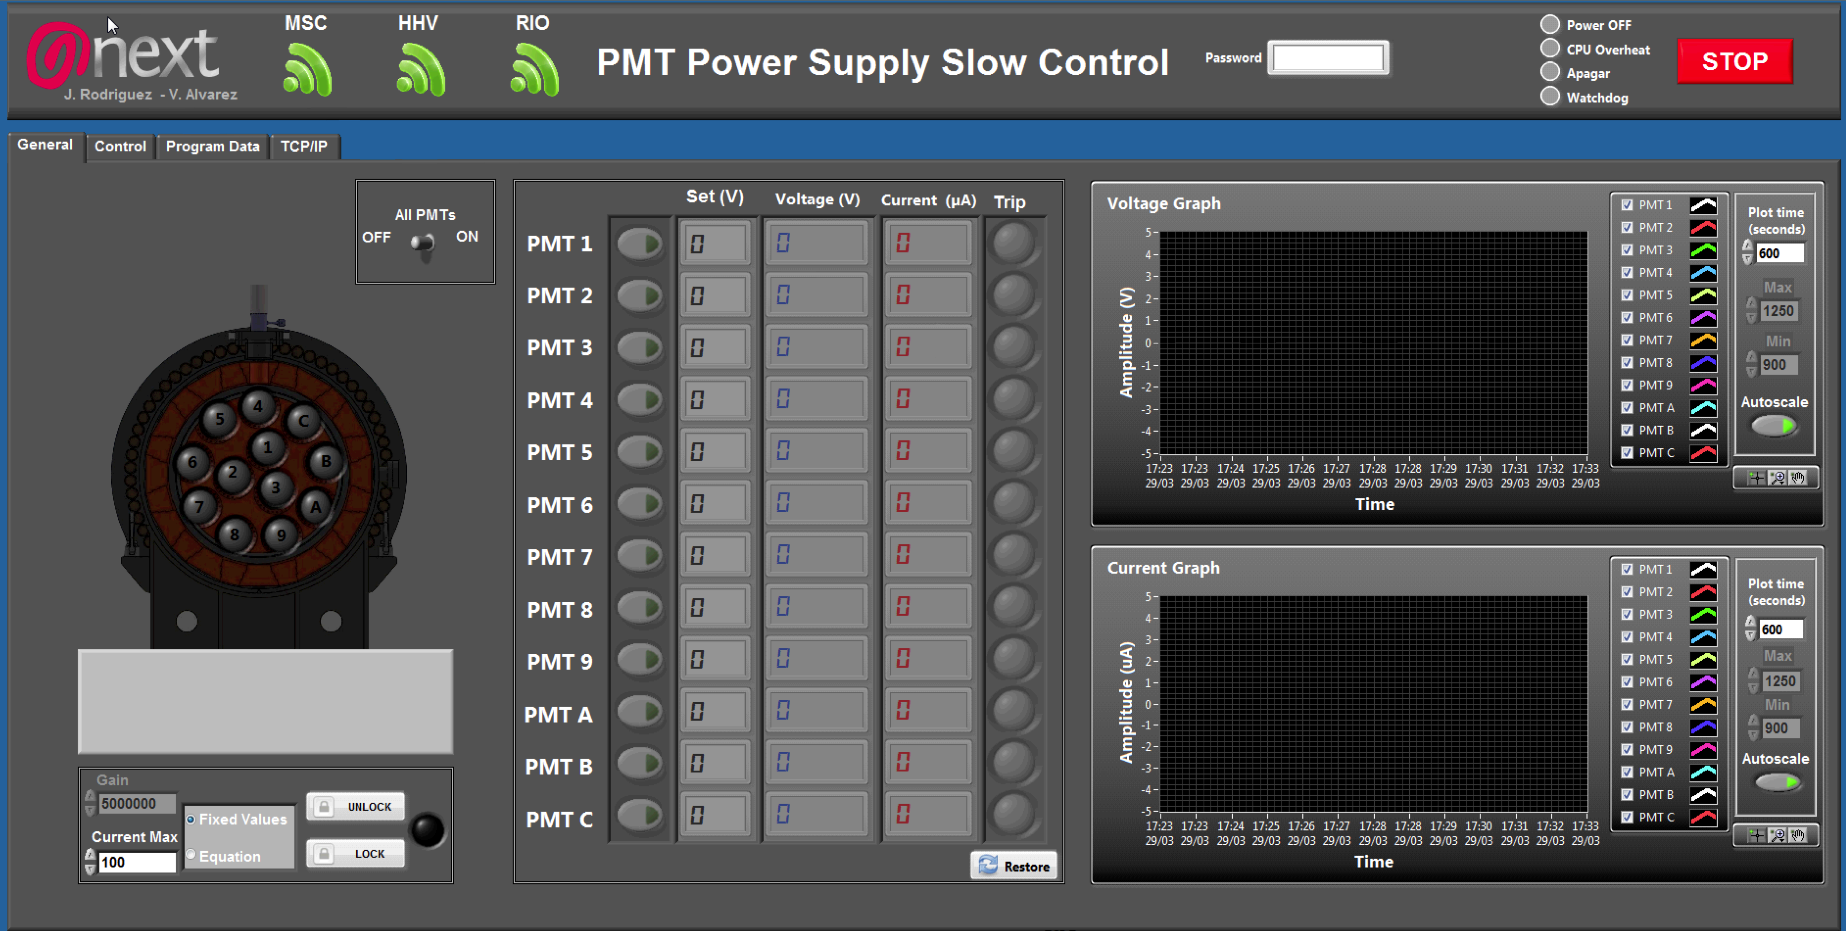
\includegraphics[width=\textwidth]{PMTs.png}}
        \caption{\textit{Screenshot of PMT power supply module for NEW}}
        \label{fig:PMT:MAIN}
    \end{center}
\end{figure}

\subsubsection*{Control}

The voltage of each PMT, email options and address can be set in this page. The events log is also is shown in this page.

\subsubsection*{Module data}

All control variables for each PMT can be set from this page.

\subsubsection*{TCP/IP}

All the parameters related to TCP/IP communication are configured here.


\subsection{HHV (Grids High Voltage Slow Control)}

This module monitors and controls the high voltage power supply for the gate and the cathode. The panel contains two tabs (see figure \ref{fig:HHV:MAIN}), one for the gate and one for the cathode, showing actual and target values as well as plots for the voltages.\\

\begin{figure}[ht]
    \bigskip
    \begin{center}\leavevmode
        \rotatebox{0}{
        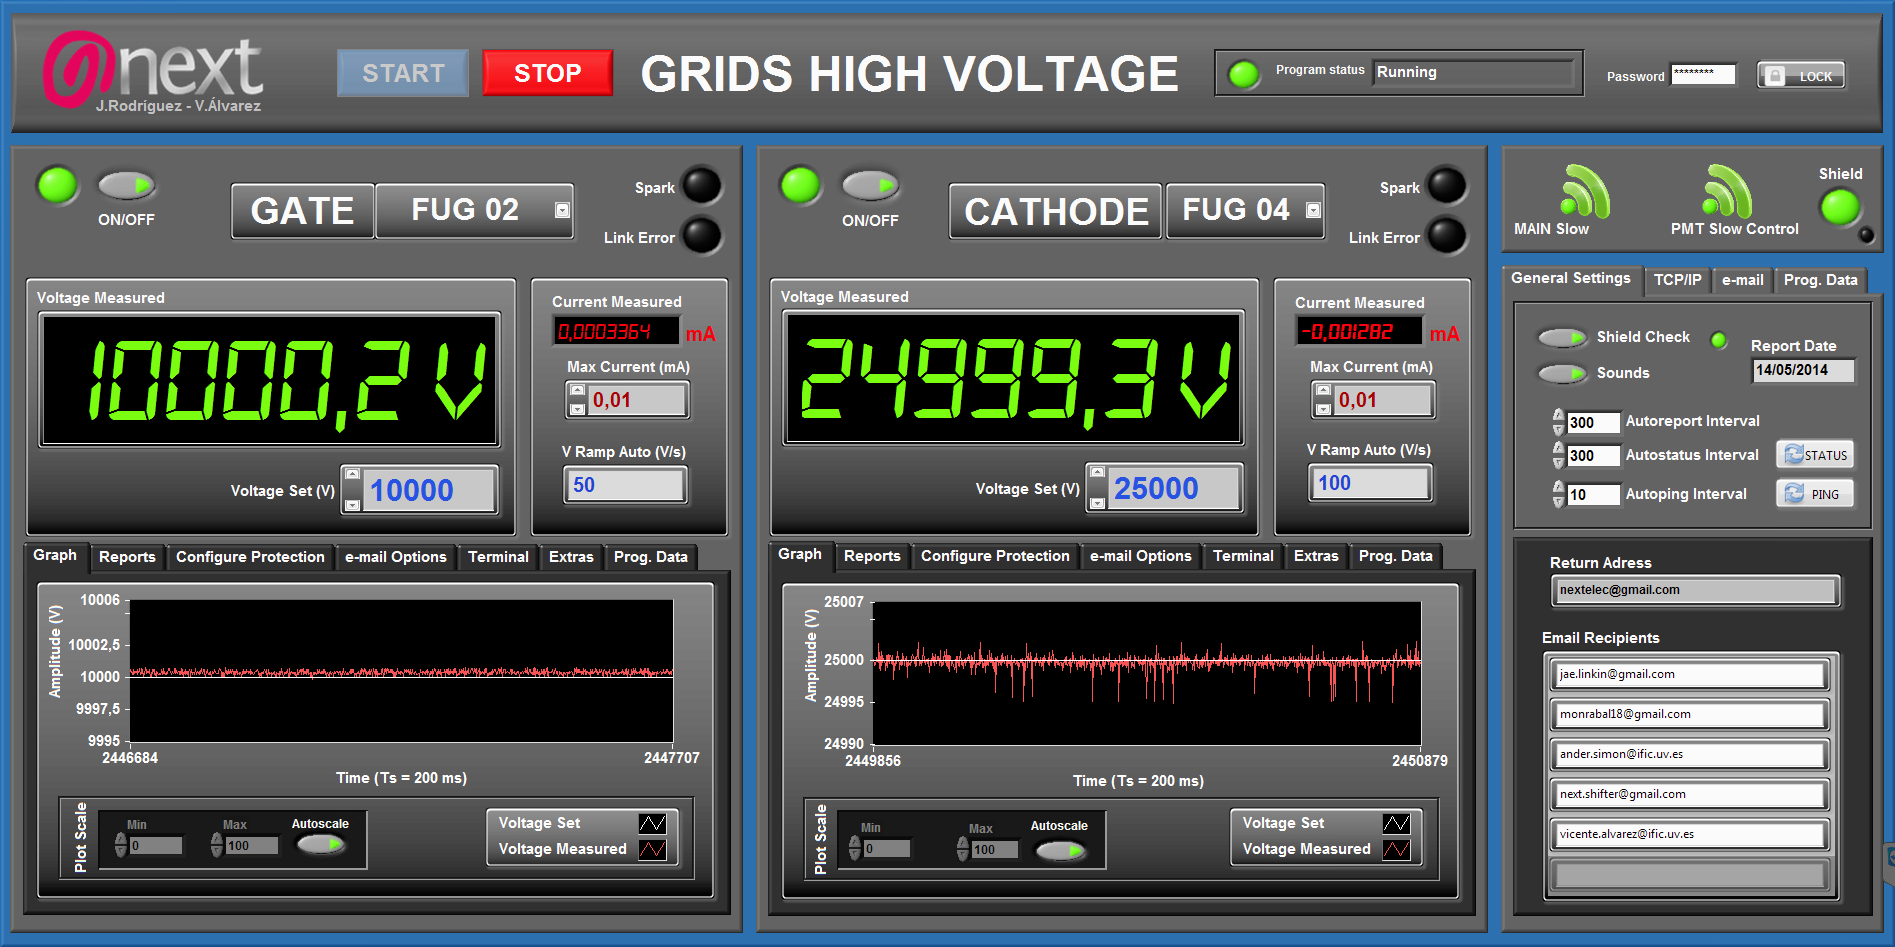
\includegraphics[width=\textwidth]{HHV.png}}
        \caption{\textit{Screenshot of Grids High Voltage module}}
        \label{fig:HHV:MAIN}
    \end{center}
\end{figure}

The module is prepared to configure the followings protection options:

\begin{itemize}
\item Time to set 0V before restore voltage (seconds).
\item Time to wait for a second spark (seconds).
\item Voltage level equivalent to OFF.
\item Second recovery time if there are sparks (seconds).
\end{itemize}

The ramp up/down time for the voltage can be configured. The conditions (like a spark or an error) that must initiate an alarm email can be set. A report can be attached to the email.

This module communicates with the PMT slow control module, PWR module and the MAIN Slow Control module. If the communication link is up and there are no failures, the indicators are green. Otherwise the indicators are grey.

The following events can trigger a message:

\begin{itemize}
\item Turning on/off the Gate or Cathode voltages.
\item Spark at Gate or Cathode.
\item Gate or Cathode recovered from spark.
\end{itemize}

A daily report shows the values of the gate and cathode voltages and currents. 

\subsection{SENSORS Slow Control}

This module monitors different temperatures and the vacuum level in the vacuum-side of the energy plane (mother-can). The vacuum is shown in a graph vs time. Figure \ref{fig:RIO:MAIN} shows a screenshot of the module's main page. 

\begin{figure}[ht]
    \bigskip
    \begin{center}\leavevmode
        \rotatebox{0}{
        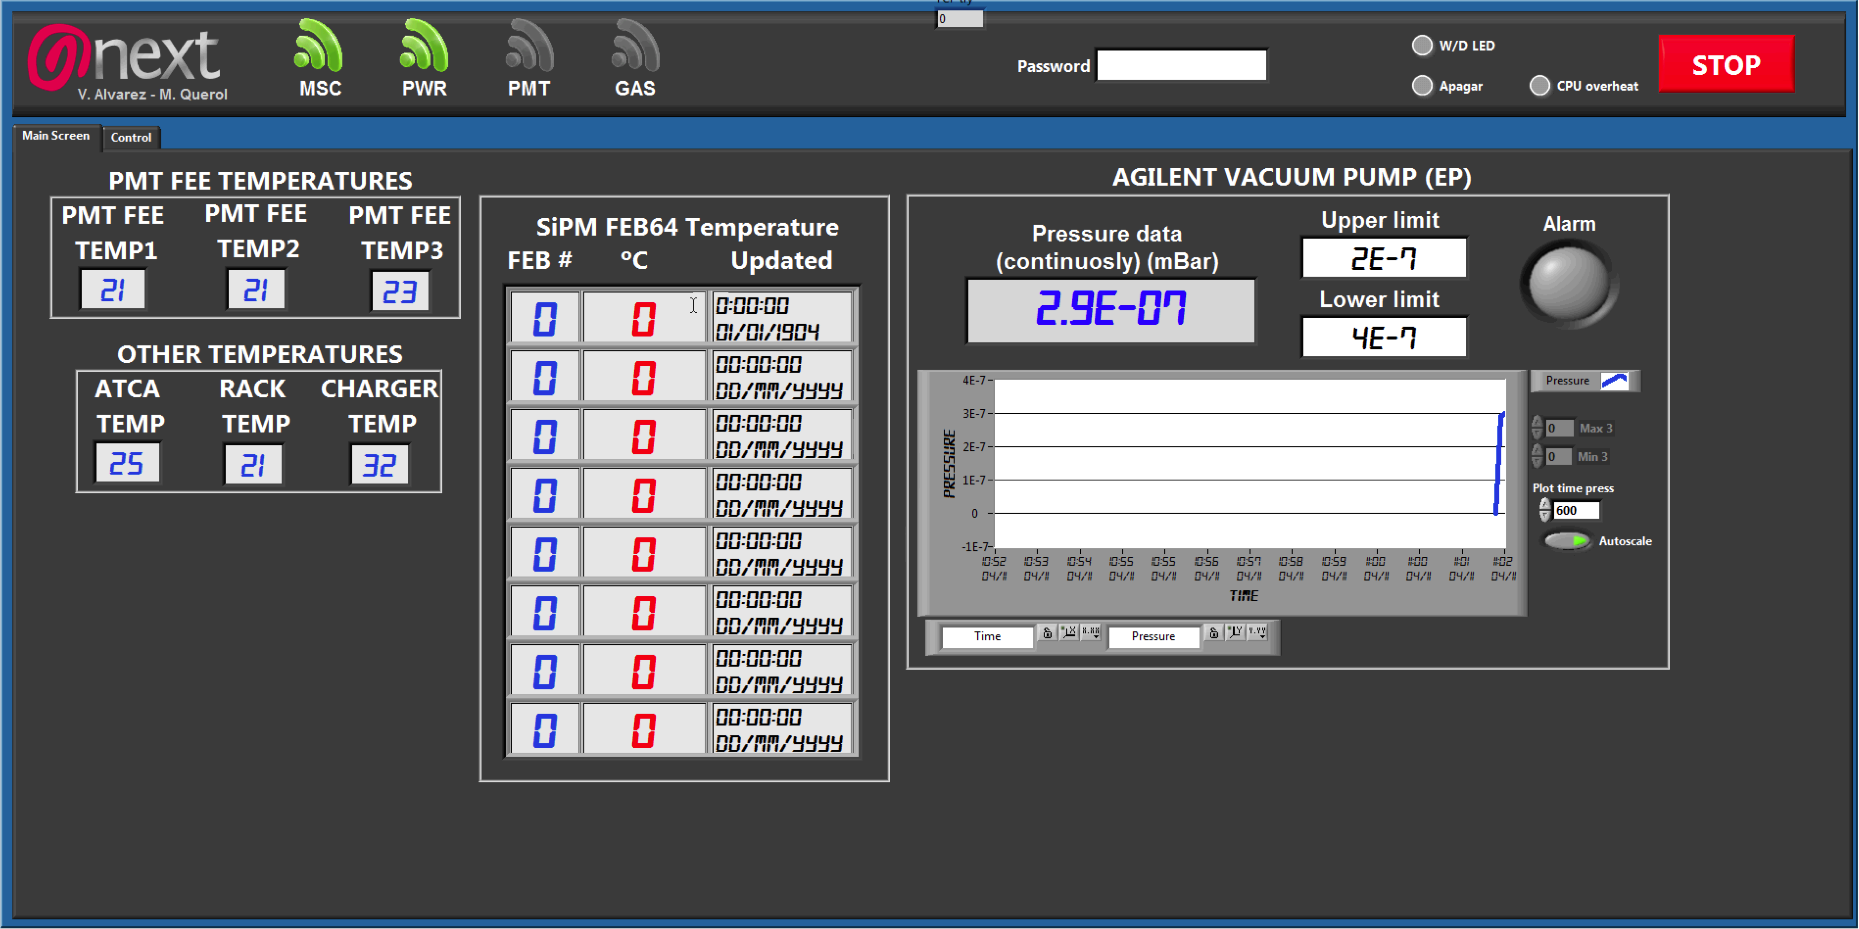
\includegraphics[width=\textwidth]{SENSORS.png}}
        \caption{\textit{Screenshot of Sensors module}}
        \label{fig:RIO:MAIN}
    \end{center}
\end{figure}


Temperature is monitored on:

\begin{itemize}
\item PMT Front-end cards (3 in total).
\item SIPM Front-end modules (28 in total).
\item ATCA chassis.
\item Energy plane electronics rack-
\item The micro-controller that turns on/off several mains AC plugs (mainly for low voltage power supplies)
\end{itemize}


The DAQ and slow control PCs can be remotely turned on from this module. The following elements can be remotely turned of/off:

\begin{itemize}
\item Tracking plane electronics rack (fan trays and power supplies).
\item ATCA chassis (DAQ).
\item PMT HV power supply.
\item Roof fan on the DAQ servers' rack.
\end{itemize}

The module communicates to Main slow Control, PMT Slow control, GAS Slow Control and PWR Slow Control via TCP/IP protocol. The module sends the status in response to a request by the Main Slow Control or when a configurable threshold is exceeded in any sensor (error condition, which also inititates an email to be sent).

A daily report is created with all the logged measurements. 

\subsection{SiPM power supplies' Slow Control}

This module monitors and controls the low-voltage power supplies for the front-end electronics and for the SiPM bias voltages. It also monitors the temperature on each Dice Board in the tracking plane.

This module communicates to the Sensors Slow Control module, GAS Slow Control module, PMT Slow Control and Main slow control module. If the communications link is up and there are no failures, the indicators are green. Indicators are grey otherwise.

PWR controls six low-voltage power supplies for the front-end electronics (Hameg HMP4040). The main page shows voltage and current displays, allows to turn on/off each power supply and has indicators showing if the power supply is turned on. As it is can be seen in figure \ref{fig:PWR:MAIN}, the sensor's bias voltage and temperature for each dice-board ais shown in a scheme that resembles their position in the NEW tracking plane. If the channel of the Dice Board is on, that Dice Board is represented in white. It is drawn in grey otherwise.

\begin{figure}[ht]
    \bigskip
    \begin{center}\leavevmode
        \rotatebox{0}{
        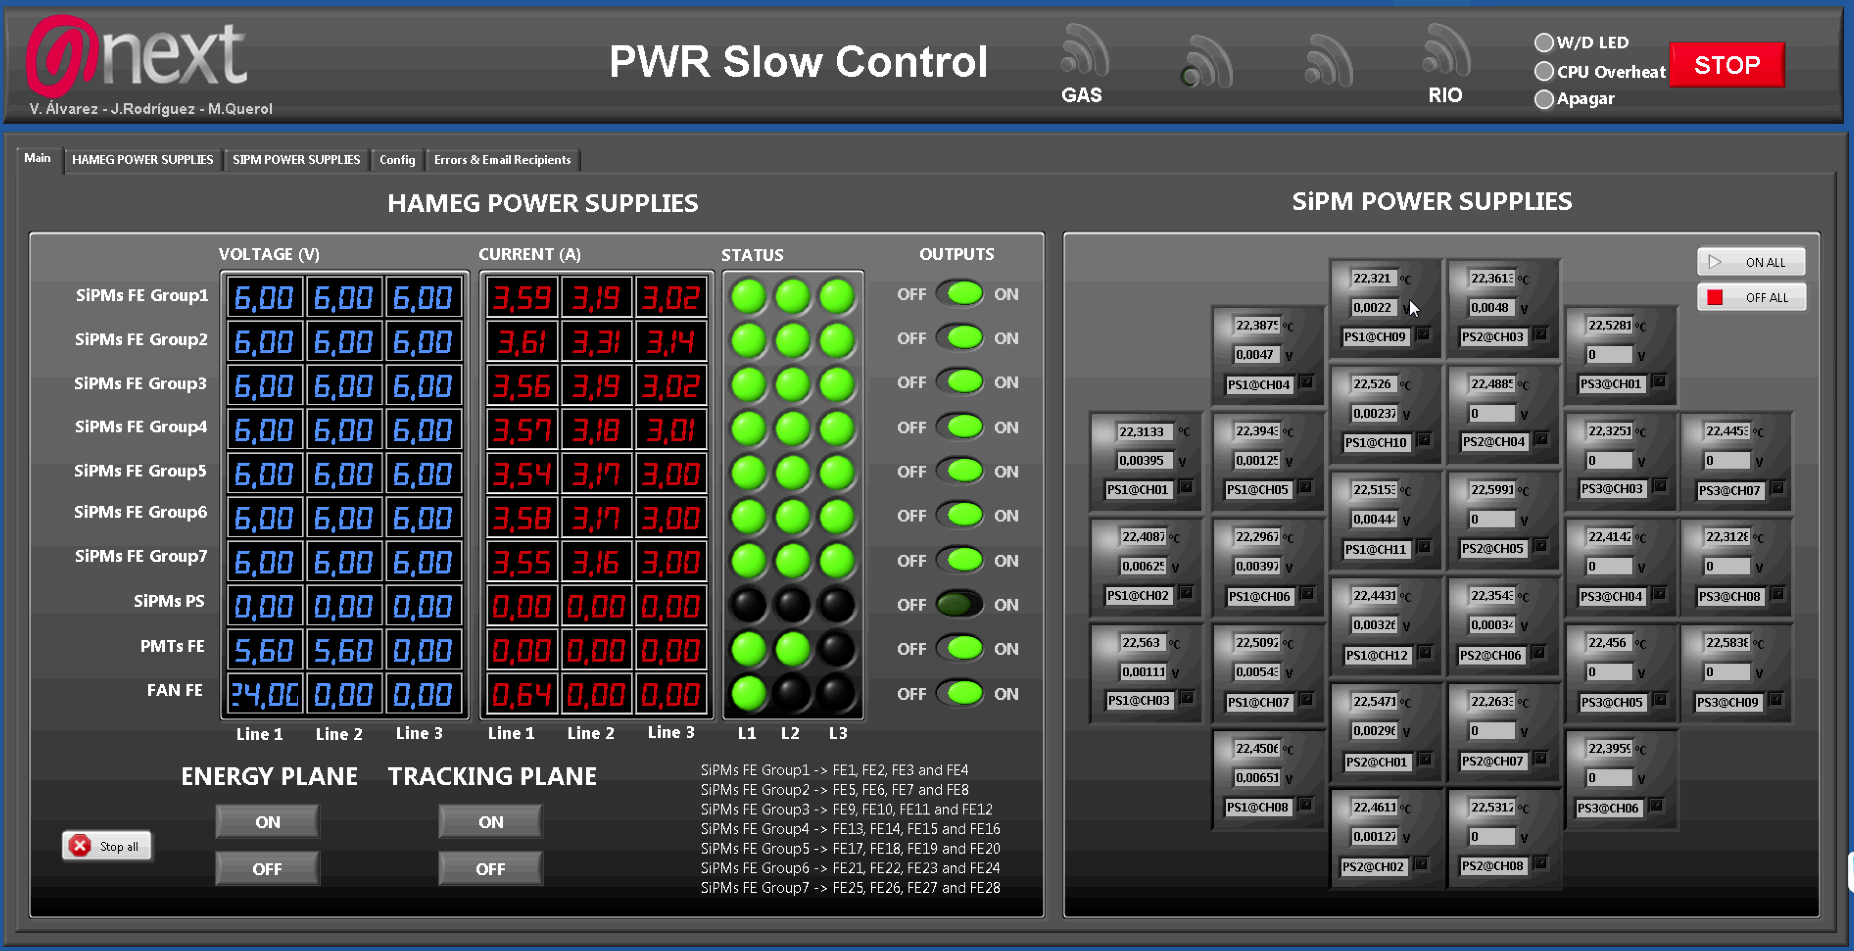
\includegraphics[width=\textwidth]{PWR.png}}
        \caption{\textit{Screenshot of PWR module}}
        \label{fig:PWR:MAIN} 
    \end{center}
\end{figure}

Manual commands that can be sent from the "SIPM PS" tab are to (1) turn on/off any channel, (2) show the parameters configured for each power supply, (3) change the voltage for a particular channel and (4) generate a report.
A graph for each power supply is shown in the "HAMEG PS" tab.

A daily report is created with all the logged measurements. 
\subsection{GAS (Gas system Slow Control)}

This module is in charge of monitoring and controlling of the gas system. 

The main page shows a scheme of the gas system with a LED on each valve that is controlled in the gas system. If the valve is open the LED is green. It the valve is closed the LED is grey. Actual values for vacuum and pressure gauges are displayed. 
This page also shows (see figure \ref{fig:GAS:GAS}) status information of the Edwards vaccuum pump (PUMP1).

\begin{figure}[ht!]
    \bigskip
    \begin{center}\leavevmode
        \rotatebox{0}{
        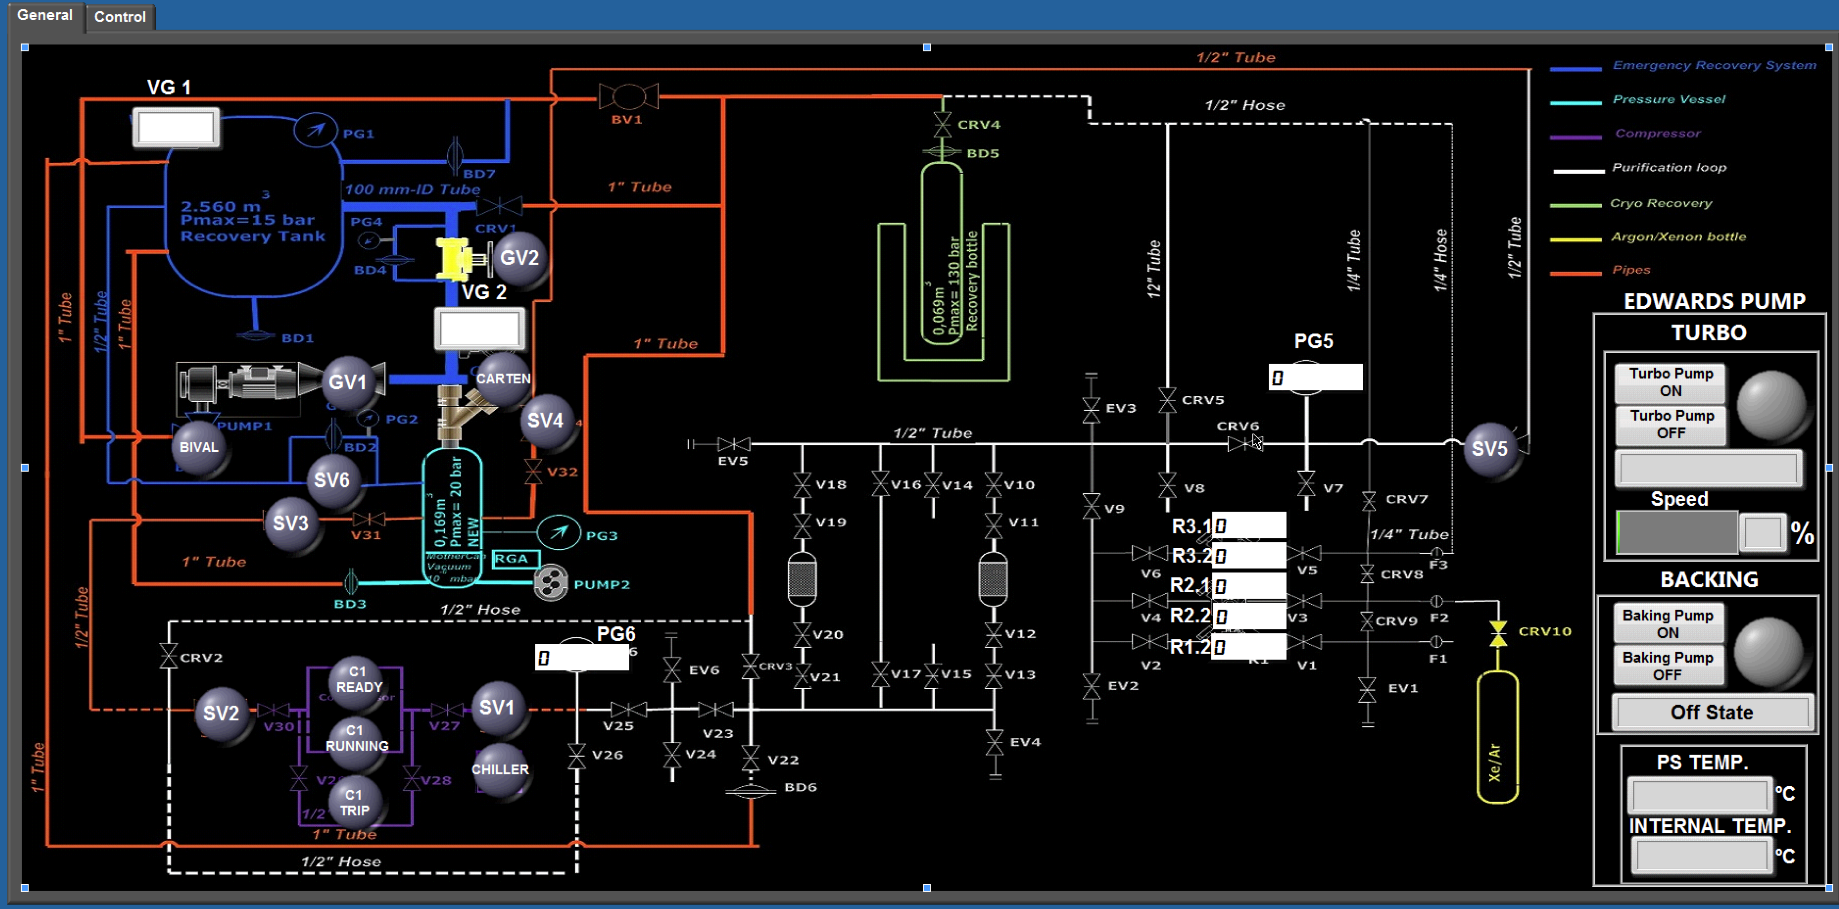
\includegraphics[width=\textwidth, ]{GAS.png}}
        \caption{\textit{Screenshot of GAS module}}
        \label{fig:GAS:GAS}
    \end{center}
\end{figure}


This communicates with the Sensors Slow Control module, PWR Slow Control module and MAIN Slow Control module. If the communication link is up and there are no errors, the indicators are green. Indicators are drawn in grey otherwise.


\subsection{MAIN Slow Control}


This software module receives, summarises and displays information from the other five modules. If the communication link is up and there are no errors, the indicators are green. Otherwise indicators appear in grey.

The main page shows whether the cathode and the gate are turned on, their voltage values and if a sparks have occurred.

It also shows the status of the PMTs. If an over-current takes place in a PMT, the PMT number and a timestamp are displayed.

A report is created with the relevant information from all slow controls modules. 

The module has a window to observe the detector via an IP camera.

The module is able to send an email alarm to the shifters. On the main screen there is an emergency button to turn off the high voltages for cathode, anode and PMTs. There is also a restore button, to restore the previous state before the emergency button was pressed. This is shown in  figure \ref{fig:MAIN:MAIN}.

\begin{figure}[ht!]
    \bigskip
    \begin{center}\leavevmode
        \rotatebox{0}{
        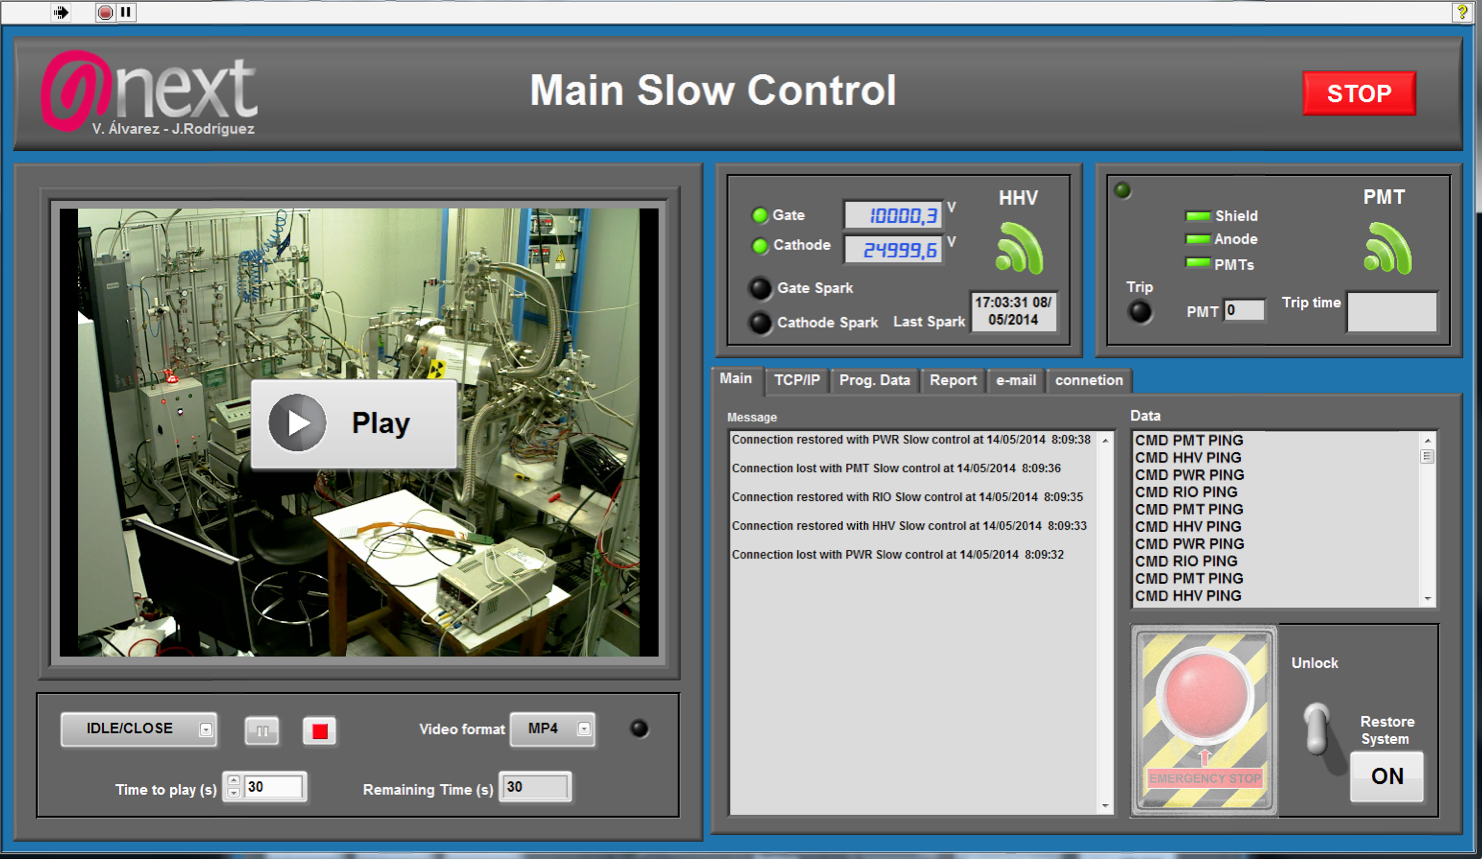
\includegraphics[width=\textwidth, ]{MAIN.png}}
        \caption{\textit{Screenshot of MAIN module}}
        \label{fig:MAIN:MAIN}
    \end{center}
\end{figure}

\subsection{FPGA module (in the cRIO chassis)}

The compactRIO is equipped with a custom FPGA Labview module. Its soft-wired logic is used to implement a robust control for the 8 defined states in the Gas System:

\begin{itemize}
\item A. Initial fill (For both Xe/Ar fills).
\item B. Normal gas re-circuation.
\item C. Normal cryogenic gas recovery (Only for Xe).
\item D. Fill from cryogenic recovery(Only for Xe).
\item E. Emergency gas dump.
\item F. Gas recovery of the emergency dump.
\item G. Saphire windows failure.
\item H. Compressor failure.
\end{itemize}


This control is posible because the cRIO is connected to the following elements (see figure \ref{fig:cRIO:cRIO}).

\begin{itemize}
\item RGA.
\item Hot getter.
\item Valves.
\item Pressure gauges.
\item Carten valve.
\item Pump2.
\item Pressure regulator.
\end{itemize}

\begin{figure}[ht!]
    \bigskip
    \begin{center}\leavevmode
        \rotatebox{0}{
        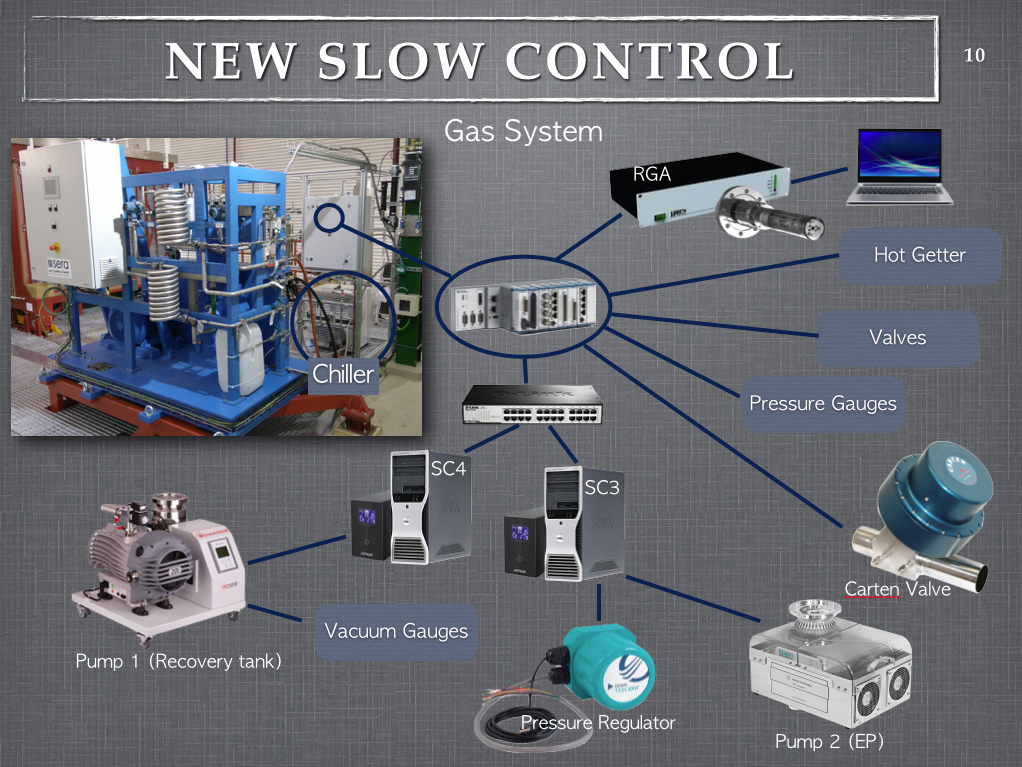
\includegraphics[width=\textwidth, ]{cRIO.png}}
        \caption{\textit{Scheme of the cRIO connections}}
        \label{fig:cRIO:cRIO}
    \end{center}
\end{figure}

\vspace{10cm}

\section{Hardware systems}

The hardware and sensors controlled from the "GAS Slow Control" Labview module are described below.

\subsection{CompactRIO \& modules}

CompactRIO is a reconfigurable embedded system for data adcquisition and control. It has a robust arcquitecture that includes an FPGA programmable via Labview. 
The different pieces of equipment in the Gas System are connected via I/O modules to the compactRIO chassis. An ethernet connection allows the chassis to interface the slow control computers. 
Figure \ref{fig:HARDWARE:RIO} shows (b) the compactRIO chassis with some I/O modules and sensors connected and (a) the slow control box called PEPON, where the compactRIO will be installed.

\begin{figure}[ht!]
  \centering
  \subfloat[\textit{PEPON}]{\label{fig:HARDWARE:PEPON}
  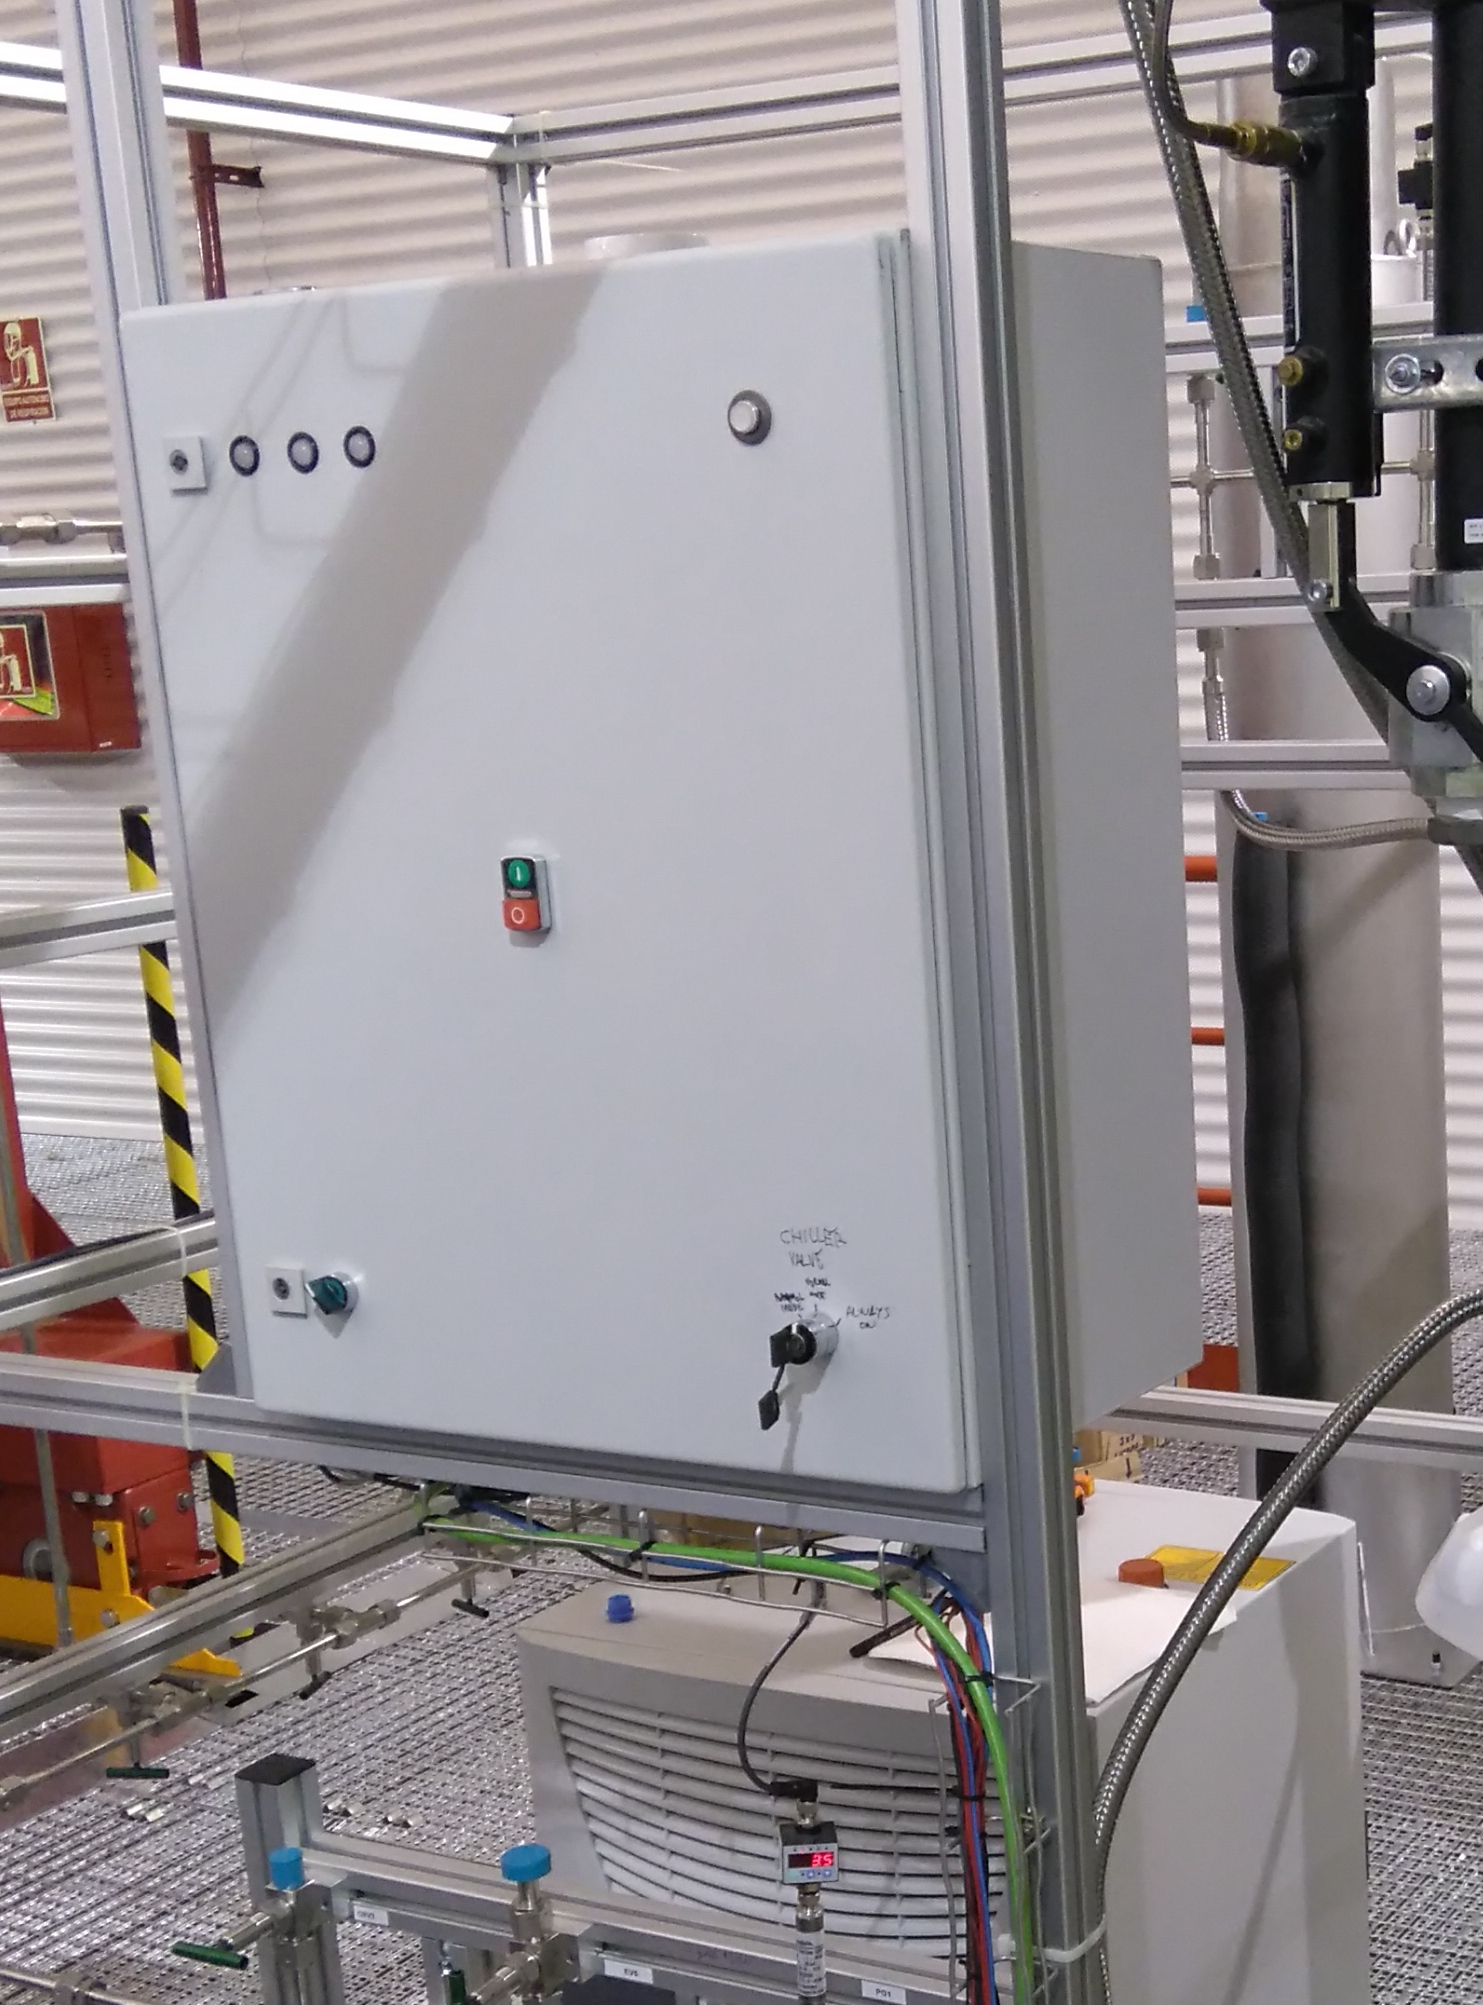
\includegraphics[width=0.5\textwidth]{PEPON.jpg}}   
  %\hspace{5mm}             
  \subfloat[\textit{compactRIO chassis}]{\label{fig:HARDWARE:cRIO}
  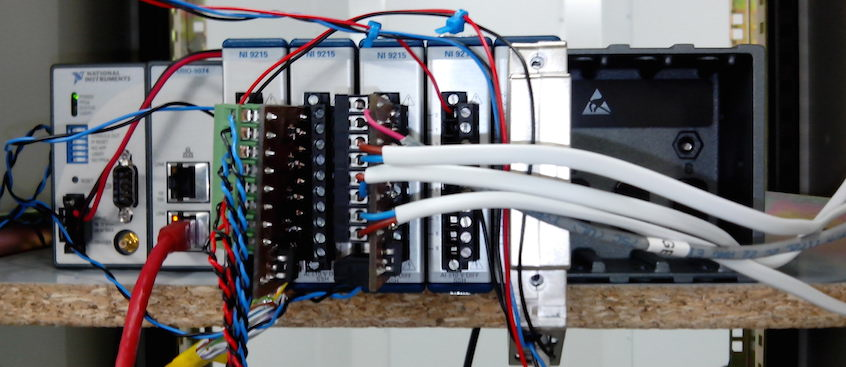
\includegraphics[width=0.5\textwidth]{cRIO_chassis.jpg}}
  \caption{\textit{PEPON and compactRIO chassis}}
  \label{fig:HARDWARE:RIO}
  \end{figure}

\subsection{Sensors, gauges \& valves}

The locations of sensors and gauges on NEW are:

\begin{itemize}
\item Temperature sensors (NTC) are located in the detector in various points, on the front-end modules, on the ATCA chassis and on the dice-boards inside the pressure vessel. 
\item Pressure gauges are located on the pressure vessel, emergency recovery tank, guillotine valve, compressor inlet and gas system pipes.
\item Vaccuum gauges are located on the emergency recovery tank, on the gas recovery conduit (vessel-recovery tank) and on the mother-can.
\end{itemize}

\section{Communication}

Most of the connections in the Control System are ethernet links in a local network. The SC2 PC (which runs the Main slow control module) is not in this local network.

Figure \ref{fig:com:com} depicts the interconnections between sensors, vacuum pumps, PCs, cRIO chassis and network switches.

\begin{figure}[ht!]
    \bigskip
    \begin{center}\leavevmode
        \rotatebox{0}{
        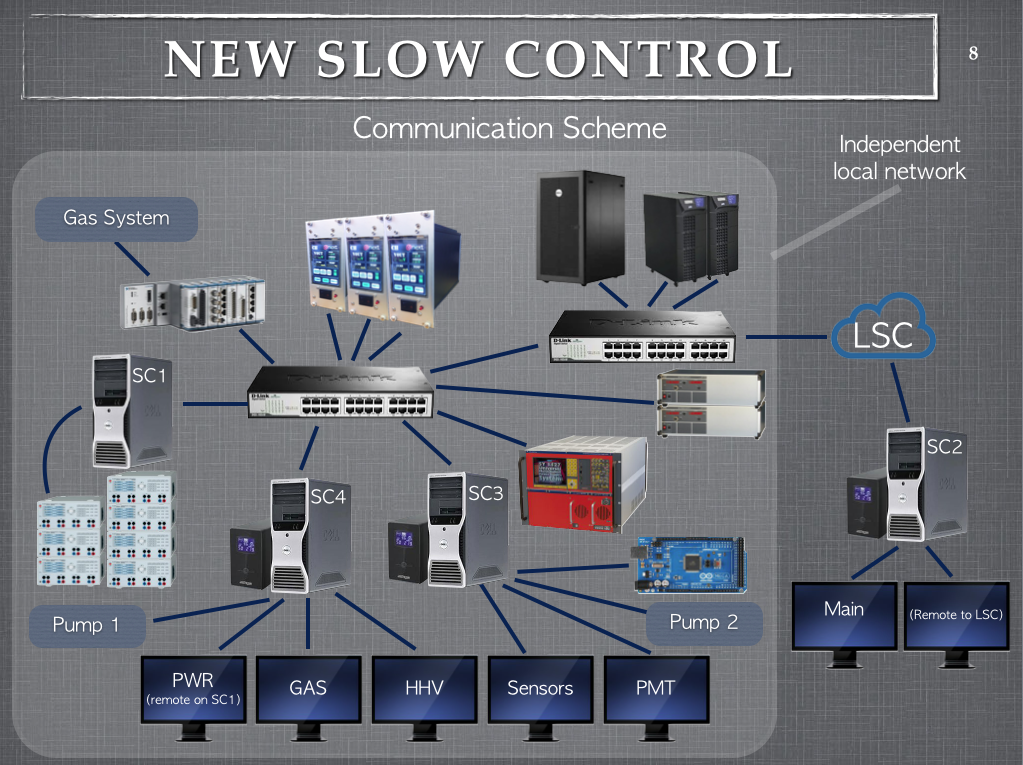
\includegraphics[width=\textwidth, ]{communication.png}}
        \caption{\textit{Scheme of the Slow control communications}}
        \label{fig:com:com}
    \end{center}
\end{figure}

\vspace{10cm}

\section{Power control}

The power control architecture is shown in figure \ref{fig:power:power}. Two large UPS provide stable power to the DAQ and storage PCs rack, to the electronics racks and to the slow control system. 
Each slow control pc has its own UPS. 

\begin{figure}[ht!]
    \bigskip
    \begin{center}\leavevmode
        \rotatebox{0}{
        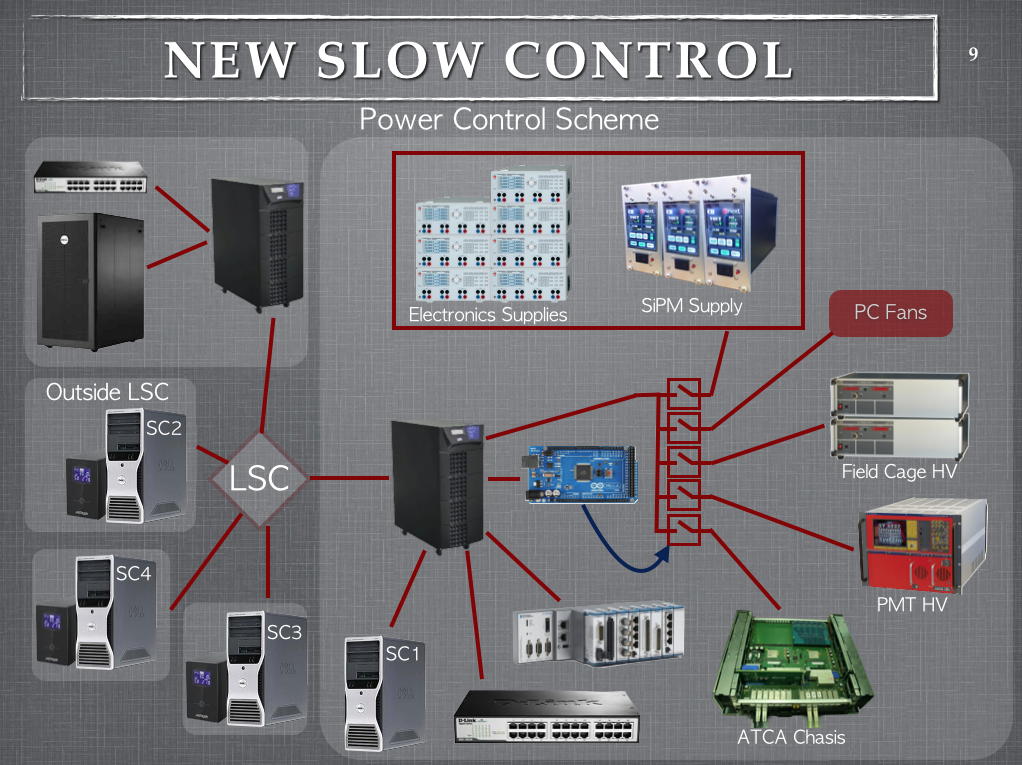
\includegraphics[width=\textwidth, ]{power.png}}
        \caption{\textit{Scheme of the power control}}
        \label{fig:power:power}
    \end{center}
\end{figure}

\section{Summary}
The Slow Control System of the NEW/NEXT detector has been described. The system is based in a configurable compact Rio module and controls all the relevant parameters for the safe operation of the apparatus, including PMT voltages, grids (cathode and gate) voltages, vacuum in the mother-can, pressure and temperature in various points and the status of the gas system. 
